\lhead{\emph{Design}}
\chapter{Design}
\label{sec:design}
In this chapter the design of the system is described. Although we have decided from the beginning to design a system based on head gestures and audio modalities, we will still discuss how alternative modalities based on existing systems and related research from chapter \ref{sec:relatedwork} would fit in a biking scenario. This will give a better insight of the importance of modality choice - the benefits and tradeoffs - when designing systems for interaction in-motion. Also the related systems could contribute to the design of specific features for our final system. This is part of the design rationale and covers the first part of this chapter. In the second part the final system design is presented.


\section{Design Rationale}
% Intro
Before choosing a design for a system different factors needs to be considered e.g. the reasons behind design decisions and the justification for it; other design alternatives considerations and the tradeoffs when choosing a design over another; the argumentation that lead to the design.

% Ubicomp challenges
When designing for ubicomp new aspects needs to be taken into consideration which increase the complexity of the system e.g. different devices, mobile users and changing environment and context \cite{barfield_fundamentals_2000}. Also we note that we are not only designing user interfaces but also the interactions between a user and the system through artifacts embedded in the environment \cite{beaudouin-lafon_designing_2004}. Furthermore it should be taken into account whether the interaction happens while the user is in motion as this introduces even more complexity as decribed earlier in section \ref{sec:interactioninmotion}.

In this project we have defined the following requirements of the system: A user should navigate a music player, or more precisely explore and select music tracks, using head gestures and audio feedback while biking. In other words we have a user interacting with artifacts, consisting of a headmounted interface and a mobile device, while biking in a traffic environment implying user awareness of road conditions, cars, other bikers, etc.

As a consequence of these requirements, we will in the next sections discuss the constraints emitting from a scenario like that and how modality combinations could fit in the design of such a system, which will lead to a discussion on related systems, that uses the audio modality as interaction form.

\subsection{Biking scenario constraints}
% intro, physical and mental constraints
Several constraints emerge from a humans capabilities to interact with a system while biking, both physically and mentally. Seen from a physical perspective the person riding the bike needs to have both hands on the handlebars in order to dodge any sudden obstructions e.g. an inattentive car. For the same reasons, and more importantly, the persons eyes needs to focus on the road. The latter is of more importance from the fact that people can not easily divide their visual attention between tasks \cite{brewster_overcoming_2002} but two hands can work independently from each other, dedicating one for steering and one for the interface. This does not mean that one hand can steer a bike perfectly - this is subjective, and we must assume that both hands for steering is preferable. Lastly biking requires the legs/feed on the pedals to move forward. From a mental perspective biking is heavily depending on the users attention or percptual load first of all to navigate the road but more importantly to keep the ability to react to traffical events. This perceptual load is complemented by the cognitive load which can increase in a very busy traffical biking scenarios and depends on the users ability to handle such scenarios.

From a system perspective a biking scenario also implies constraints. First of all interaction with the system should preferably go through some kind of wearable device or at least something easy installable hardware that could be attached to the bike. The system also needs to optimize handling of unintentional interaction during biking e.g. motion gestures when riding a bumpy road. Secondly and most important the system needs to aim for minimizing the workload required by the user - every added feature should be considered i.e. every interaction task should be considering conducted while biking. Also the content presented to the user should be considered in terms of the interaction modality being used e.g. in a visual music player interface artist/track information and a lot of navigation possibilities might be good but if the same information and functionality were to provided via audio this would cause a non-linear effect and add complexity to the system.

\subsection{Modalities reasoning}

% HMD, Gaze tracking
\textbf{Visual challenges}

A headmounted visual display like Google Glass would give total hands-freeness when biking but as mentioned in \ref{sec:interactioninmotion} such displays can be hard and obtrusive to use in bright daylight. Also such interface still would require the visual attention from the user \cite{geelhoed_safety_2000}, although the user would not have to change head direction while biking (like when looking down on a traditional stop-to-interact interface). Same arguments follows with a gaze tracking solution. Also such a solution could require some kind of installation on the bike e.g. a camera attached to the handlebars for tracking the eye. Mobile solutions exists \cite{mardanbegi_eye-based_2012} but this will still imply the user to look at the device, and probably hold the device i.e. occupying one hand, while interacting. However the benefit with using visual displays like the headmounted displays in our scenario is, that it's possible to keep the rich visual experience of exploring music tracks before selecting them, linearly translated from the stop-to-interact music player interfaces. It can be argued though, that the experience is not as rich when biking in a traffic environment where attention is divided.

Studies on multimodal interaction \cite{zhao_shared_2013} have shown that when humans needs to attend a physical visual task and a virtual task at the same time (dual task situation) - they found it significantly distractive to attend to the virtual task in a visual way. Instead audio has shown to be less distractive. The biking while interacting scenario can easily be translated into such a dual task where the physical task is to attend to the road and traffic and virtual task is to explore and select music tracks. Inspired from this and from other studies showing that audio can improve usability with mobile devices in eyes-free mobile conditions \cite{brewster_multimodaleyes-freeinteraction_2003}, we will consider systems designs that uses audio modalities next.

% Audio interfaces/related systems
\textbf{Audio modality combinations}




% Thomas comment:
% i recommend to start the system design discussion from the constraints emerging from human capabilties to interact with a system while biking. all possible input and output modalities should be explored and then, finally, you should land in suggesting a head-gesture based UI.

% Biking scenario:
% Human constraints: Physical, Mental, Environment

% Modalities in biking scenario, pros, cons:
% Vision: HMDs, Gaze tracking
% Speech: Speech recognition, simple commands, environmental noise
% Gestures: Hand, Head, Leg, Body pose
% Audio

% Related systems

% From theory:
% - Modality replacement linear effect (from visual overview to ?)

% Headset controller: 
% This kind of interaction though assumes the user has created a playlist and knows in which order the tracks follows to navigate efficiently to the wanted track. Also this kind of menu is 1-dimensional in the sense that tracks needs to be placed in a sequence missing the opportunity to go into a submenu e.g. an album of an artist. It should also be taken into account that although only using one hand for interaction this could still create challenges e.g. when steering or hitting the breakes while biking could require both hands on the steering.

% Voice recognition:
% ...In this application example the user could express simple commands like play, stop, next/previous track and queue. Voice recognition however introduces accuracy and stability challenges especially in mobile noisy environments. At the same time speech commands are limited - it would introduce even more complexity if the system should be able to interpret detailed commands e.g. an artist name or even a track title.
% - good ref about speech recognition challenges \cite{sawhney_nomadic_2000}


%- Unintentional behaviour e.g. activating menu biking over a bump or a sudden need for rotating head because of obstacles
%- Weather conditions, too much wind disrupting the audio, rain on headset
%- Noise can disrupt audio


\subsection{Auditory menus}
...


\section{Spatial Music Menu}
This section contains a description of the system design.

\subsection{Soundscape}
- Music, strength of recognizing artist/track through listening vs seeing the text on a screen
- Horizontal argument
- Two menu interaction modes, distance/
- Selective attention task
- Simultanous sounds, exploring, cocktail party effect argument
- Experimental design, sounds perceived, zoom effect, user should detect sound direction (which track)

Metaphor: Carousel

Soundscape design illustration, figure \ref{fig:sounddesign}

\begin{figure}[t]
	\centering
		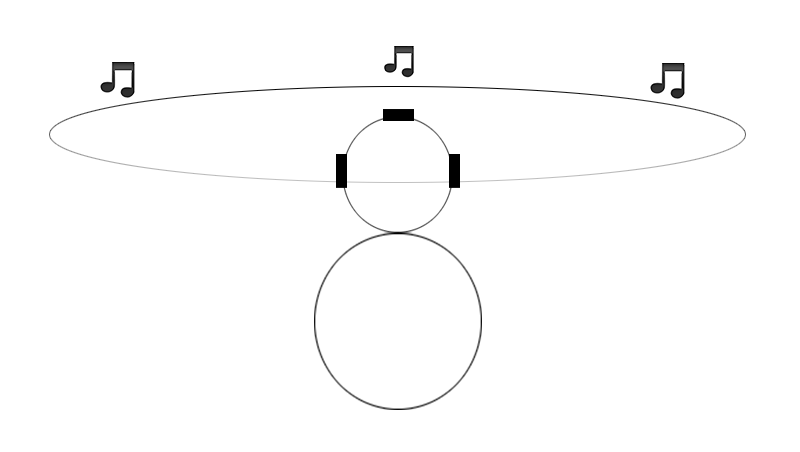
\includegraphics[width=0.6\textwidth,height=\textheight,keepaspectratio]{./Figures/sounddesign.png}
		\rule{35em}{0.5pt}
	\caption[Soundscape Design]{Soundscape Design - Visualising how the circular auditory menu surrounds a person (viewed from the persons back)}
	\label{fig:sounddesign}
\end{figure}

\subsection{Navigation}
- Adaption of real world music player menu
- Figure showing levels of menu
- Navigation
- Head gestures
- Activating menu
- Feedback when gesture recognized
- Nod = yes

Several studies show that circular auditory menus are the way to go because of horizontally positioned sounds (ref?)





























% OLD - Use some parts here and move some to introduction method section
\begin{comment}

This chapter first explains the design methods used and the most important design activities and choices made in the design process. Based on this process the final prototype design is presented at the end of the chapter.

\section{Design model and methods}
In this section the model used for designing the final prototype is presented including the different techniques used throughout the design process.

The related works conducts the foundations for an early first prototype. This prototype will then go through an iterative design process, taking a user centered approach. This will enable specifications to emerge during the process and these learnings and modifications will result in new experiments and prototypes. This iterative design model is illustrated in figure \ref{fig:iterative}.

\begin{figure}[t]
	\centering
		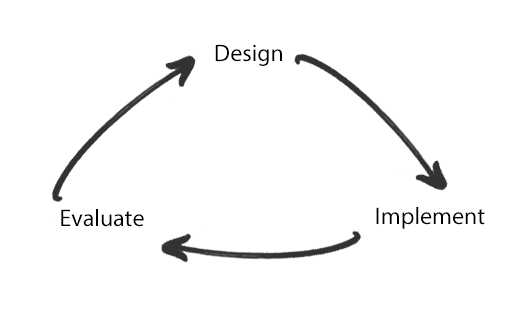
\includegraphics[width=0.6\textwidth,height=\textheight,keepaspectratio]{./Figures/iterative.png}
		\rule{35em}{0.5pt}
	\caption[Iterative Design Model]{Iterative Design Model}
	\label{fig:iterative}
\end{figure}

\subsection{Envisionment}
One of the goals with the final system is that it should be eyes-free i.e. the user should not depend on a visual screen UI at the end. Despite this goal, the use of a screen to visualize e.g. a virtual menu, can be helpful in the design process. This will enable test users to get a quicker and better understanding of how the interaction works. In this design process a mobile device screen will be used for envisionment - this is also called a hifi prototype or software prototype \cite{benyon_designing_2010}.

More concretely audio sources and the users head position including rotation will be mapped visually to a screen dynamically during user interaction. An example of this screen is shown in figure ?

\section{Design process}
This section starts out by describing the first experimental prototype design inspired from previous research work and then each iteration including user feedback and design changes and experiments. More specifically the design completed 2 iterations before the final prototype design.

\subsection{Initial prototype design considerations}
Before we started to reason about initial design choices we started out by defining what the system actually needed in order to evaluate and revise the hypothesis from the problem statement.

% intro, track exploring
First of all we wanted the system to be able to play music. This is in itself a trivial task but as we the same time wanted to control the system only with with head gestures and audio output a traditional music player includes too many options e.g. play, pause, stop, next/previous, volume, equalizer, track exploring, etc for the scope of this thesis. All the alternative music players mentioned in chapter \ref{sec:relatedwork} is limited to simple commands like play, stop, next/previous and volume. Taking it a step further we wanted to evaluate the track exploring part i.e. navigating to a preferred track and playing it. This made et clear that some kind of auditory menu with tracks as menu items was needed and although not music players the related systems from chapter \ref{sec:relatedwork} using auditory menus could inspire to an intital menu design.

% Auditory menu, exocentric, head rotation constraints
When looking at the different related auditory menu designs we needed to find a design that fitted into the context of the user activity i.e. biking and also user interaction modality. E.g. in a biking scenario the user should have eyes on the road thereby constraining the head rotation. Park et. al \cite{park_gaze-directed_2011} showed good results with a 2D grid menu. It should be taken into account that their audio output consists of simple speech commands e.g. speech recorded numbers. We want to present multiple music streams (non-speech audio) and studies have shown that when presenting multiple non-speech audio streams simultanously in a spatial audio space, segregating the audio streams horizontically has a better effect than vertical alignment [TODO: ref]. It seemed that a circular auditory menu could be a good starting point and both Kajastila and Lokki \cite{kajastila_interaction_2013} and also Brewster et. al \cite{brewster_multimodaleyes-freeinteraction_2003} evaluated this kind of menu design with good results.

[TODO: Image/prototype sketch?]

% Circular menu design, head gestures
While placing music streams in a circular way around a users audio space we needed a way of navigating to and chosing a specific track. The Brewster et. al \cite{brewster_multimodaleyes-freeinteraction_2003} system uses directed nods to choose an item but this limits the number of items to 4 (1 for every 90 degrees) as a nod in 45 degrees

The inititial interaction design was inspired from Kajastila and Lokkis system although they used hand gestures as modality input. 

For navigating and choosing menu items

[TODO: egocentric vs exocentric audio output, Brewster system good ref \cite{vazquez-alvarez_eyes-free_2011}]

% Summarising

[TODO]
In this project multiple audio sources (music tracks) are presented for the user at the same time but none of them requires a respond i.e. the focus is on selective-attention tasks.

\end{comment}





% OLD


% From wiki:
% - the reasons behind a design decision,
% - the justification for it,
% - the other alternatives considered,
% - the trade offs evaluated, and
% - the argumentation that led to the decision.









